\documentclass{beamer}
\usepackage[utf8]{inputenc}

\usetheme{Madrid}
\usecolortheme{default}
\usepackage{amsmath,amssymb,amsfonts,amsthm}
\usepackage{txfonts}
\usepackage{tkz-euclide}
\usepackage{listings}
\usepackage{adjustbox}
\usepackage{array}
\usepackage{tabularx}
\usepackage{gvv}
\usepackage{lmodern}
\usepackage{circuitikz}
\usepackage{tikz}
\usepackage{graphicx}

\setbeamertemplate{page number in head/foot}[totalframenumber]

\usepackage{tcolorbox}
\tcbuselibrary{minted,breakable,xparse,skins}



\definecolor{bg}{gray}{0.95}
\DeclareTCBListing{mintedbox}{O{}m!O{}}{%
  breakable=true,
  listing engine=minted,
  listing only,
  minted language=#2,
  minted style=default,
  minted options={%
    linenos,
    gobble=0,
    breaklines=true,
    breakafter=,,
    fontsize=\small,
    numbersep=8pt,
    #1},
  boxsep=0pt,
  left skip=0pt,
  right skip=0pt,
  left=25pt,
  right=0pt,
  top=3pt,
  bottom=3pt,
  arc=5pt,
  leftrule=0pt,
  rightrule=0pt,
  bottomrule=2pt,

  colback=bg,
  colframe=orange!70,
  enhanced,
  overlay={%
    \begin{tcbclipinterior}
    \fill[orange!20!white] (frame.south west) rectangle ([xshift=20pt]frame.north west);
    \end{tcbclipinterior}},
  #3,
}
\lstset{
    language=C,
    basicstyle=\ttfamily\small,
    keywordstyle=\color{blue},
    stringstyle=\color{orange},
    commentstyle=\color{green!60!black},
    numbers=left,
    numberstyle=\tiny\color{gray},
    breaklines=true,
    showstringspaces=false,
}
%------------------------------------------------------------
%This block of code defines the information to appear in the
%Title page
\title %optional
{4.13.100}
\date{\today}
%\subtitle{A short story}

\author % (optional)
{Shivam Sawarkar \\ AI25BTECH11031}



\begin{document}


\frame{\titlepage}
\begin{frame}{Question}
    Let $\vec{S}$ be the reflection of a point $\vec{Q}$ with respect to the plane given by $\vec{r}=-(t+p)\hat{i}+t\hat{j}+(1+p)\hat{k}$ where $t$, $p$ are real parameters and $\hat{i}$, $\hat{j}$, $\hat{k}$ are the unit vectors along the three positive coordinate axes. If the position vectors of $\vec{Q}$ and $\vec{S}$ are $10\hat{i}+15\hat{j}+20\hat{k}$ and $\alpha\hat{i}+\beta\hat{j}+\gamma\hat{k}$ respectively, then which of the following is/are TRUE ? \\ 
\begin{enumerate}[a]
    \item $3(\alpha+\beta) = -101$
    \item $3(\beta+\gamma) = -71$
    \item $3(\gamma+\alpha) = -86$
    \item $3(\alpha+\beta+\gamma) = -121$
\end{enumerate}
\end{frame}

\begin{frame}{Soluion}
    The plane is given by 
\begin{align}
\vec{r} = t\myvec{-1 \\ 1 \\ 0}+p\myvec{-1 \\ 0 \\ 1}+\myvec{0 \\ 0 \\ 1}
\end{align} 
so two direction vectors are
\begin{align}
\vec{u} = \myvec{-1\\1\\0}, 
\qquad 
\vec{v} = \myvec{-1\\0\\1}.
\end{align}

Hence the normal vector is
\begin{align}
\vec{n} = \vec{u} \times \vec{v} 
= \myvec{1\\1\\1}.
\end{align}


So the plane equation becomes
\begin{align}
\vec{n}^\top\vec x = 1.
\end{align}
\end{frame}

\begin{frame}{Solution}
    For a point $\vec q \in \mathbb{R}^3$, its reflection across the plane 
$\vec{n}^\top\vec{x} = 1$ is
\begin{align}
\vec{S} = \vec{Q}-2\frac{\vec{n}^\top\vec{Q}-1}{\norm{n}^2}\vec{n},
\end{align}

Here
\begin{align}
\vec{n} = \myvec{1\\1\\1},  
\quad \vec{Q} = \myvec{10\\15\\20}.
\end{align}

\begin{align}
\vec{n}^\top\vec n = 1^2+1^2+1^2=3.
\end{align}


\begin{align}
\vec{S}=\myvec{\alpha \\ \beta \\ \gamma} = \myvec{\frac{58}{3} \\ -\frac{43}{3} \\ -\frac{28}{3}}.
\end{align}
\end{frame}

\begin{frame}{Solution}
    \begin{align}
3(\alpha+\beta) = -101,\quad
3(\beta+\gamma) = -71,\quad
3(\gamma+\alpha) = -86,\quad
3(\alpha+\beta+\gamma) = -129.
\end{align}

Hence, the correct options are
\begin{align}
\boxed{(a), (b), (c)}.
\end{align}
\end{frame}

\begin{frame}{Plot}
    \begin{figure}
        \centering
        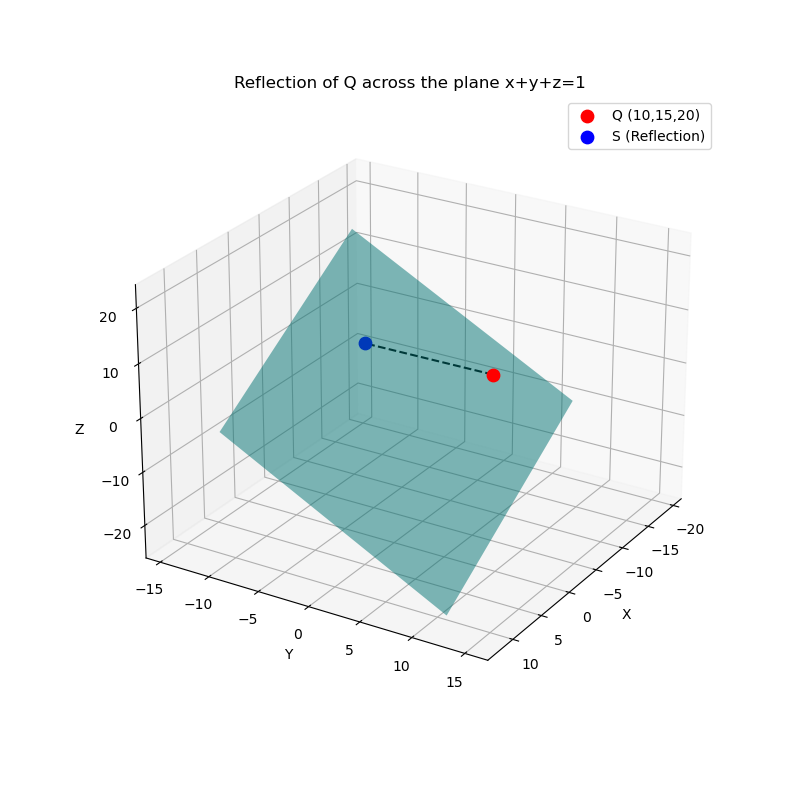
\includegraphics[width=0.5\linewidth]{figs/plot10.png}
        \caption{}
        \label{fig:placeholder}
    \end{figure}
\end{frame}

\begin{frame}[fragile]{C Code}
    \begin{verbatim}
#ifndef REFLECTION_H
#define REFLECTION_H

#include <stdio.h>

// Function to compute reflection of a point (x,y,z)
// across the plane x+y+z=1.
// The result is stored in (alpha, beta, gamma).
void reflect_point(double x, double y, double z,
                double *alpha, double *beta, double *gamma) {
    double n[3] = {1.0, 1.0, 1.0};   
    double d = 1.0;                  
    double norm_sq = 3.0;
    \end{verbatim}
\end{frame}

\begin{frame}[fragile]{C Code}
    \begin{verbatim}
    // Dot product n.q
    double dot = n[0]*x + n[1]*y + n[2]*z;

    // Reflection formula: s = q - 2((n.q - d)/||n||^2) * n
    *alpha = x - 2.0*(dot - d)/norm_sq * n[0];
    *beta  = y - 2.0*(dot - d)/norm_sq * n[1];
    *gamma = z - 2.0*(dot - d)/norm_sq * n[2];
}

#endif
    \end{verbatim}
\end{frame}

\begin{frame}[fragile]{C Code}
    \begin{verbatim}
#include "solution.h"

int main() {
    double x, y, z;
    double alpha, beta, gamma;

    printf("Enter coordinates of Q (x y z): ");
    scanf("%lf %lf %lf", &x, &y, &z);
    reflect_point(x, y, z, &alpha, &beta, &gamma);
    printf("Reflected point S = (%.6lf, %.6lf, %.6lf)\n", alpha, beta, gamma);

    return 0;
}
    \end{verbatim}
\end{frame}

\begin{frame}[fragile]{Python Code}
    \begin{verbatim}
import numpy as np

def reflect_point(x, y, z):
    n = np.array([1.0, 1.0, 1.0])
    d = 1.0  # plane constant
    norm_sq = np.dot(n, n)  # = 3
    q = np.array([x, y, z])
    dot = np.dot(n, q)
    s = q - 2 * (dot - d) / norm_sq * n
    return s

    x, y, z = map(float, input("Enter coordinates of Q (x y z)
    : ").split())
    alpha, beta, gamma = reflect_point(x, y, z)
    print(f"Reflected point S = ({alpha:.6f}, {beta:.6f},
    {gamma:.6f})")
    \end{verbatim}
\end{frame}

\begin{frame}[fragile]{Python + C Code}
    \begin{verbatim}
import ctypes

# Load the shared library
lib = ctypes.CDLL("./solution.so")

# Define argument and return types for the function
lib.reflect_point.argtypes = [ctypes.c_double, ctypes.c_double,
ctypes.c_double,
                        ctypes.POINTER(ctypes.c_double),
                      ctypes.POINTER(ctypes.c_double),
                      ctypes.POINTER(ctypes.c_double)]

def reflect_point(x, y, z):
    alpha = ctypes.c_double()
    beta  = ctypes.c_double()
    gamma = ctypes.c_double()
    \end{verbatim}
\end{frame}

\begin{frame}[fragile]{Python + C Code}
    \begin{verbatim}
    lib.reflect_point(x, y, z,
                      ctypes.byref(alpha),
                      ctypes.byref(beta),
                      ctypes.byref(gamma))
    return alpha.value, beta.value, gamma.value


# --- Main ---
if __name__ == "__main__":
    x, y, z = map(float, input("Enter coordinates of Q (x y z):
    ").split())
    alpha, beta, gamma = reflect_point(x, y, z)
    print(f"Reflected point S = ({alpha:.6f}, {beta:.6f},
    {gamma:.6f})")
    \end{verbatim}
\end{frame}






\end{document}